% !TEX program = xelatex
\documentclass[12pt,a4paper,oneside]{report}
\usepackage[T1]{fontenc}
\usepackage{lmodern}
\usepackage[a4paper,left=28mm,right=25mm,top=25mm,bottom=25mm,headheight=15pt]{geometry}
\usepackage{amsmath,amssymb,graphicx,booktabs,tabularx,array,multirow}
\usepackage{xcolor,setspace,fancyhdr,titlesec,caption,subcaption,enumitem}
\usepackage{tikz}
\usetikzlibrary{arrows.meta,positioning,shapes.geometric,calc}
\usepackage{microtype}
\usepackage{placeins,float}
\usepackage[numbers,sort&compress]{natbib}
\usepackage[hidelinks,bookmarksnumbered,hypertexnames=false,pdfauthor={Ayush Goel},pdftitle={Patient-Level Glioma Grade Classification from Multimodal 3D MRI}]{hyperref}
\usepackage{bookmark}
\makeatletter
\let\tableinput\@@input
\makeatother
\definecolor{navy}{HTML}{19344B}
\definecolor{teal}{HTML}{167D9A}
\definecolor{pale}{HTML}{EEF4F7}
\setstretch{1.18}
\setlength{\parindent}{1.2em}
\setlength{\parskip}{4pt}
\setlength{\emergencystretch}{2em}
\raggedbottom
\brokenpenalty=10000
\clubpenalty=10000
\widowpenalty=10000
\setcounter{tocdepth}{1}
\setcounter{secnumdepth}{2}
\captionsetup{font=small,labelfont=bf,labelsep=period,skip=8pt}
\captionsetup[table]{position=top}
\setlist{itemsep=3pt,topsep=5pt,leftmargin=1.6em}
\renewcommand{\arraystretch}{1.22}
\newcolumntype{Y}{>{\raggedright\arraybackslash}X}
\newcommand{\roi}{\ensuremath{96\times96\times96}}
\newcommand{\model}{\textsc{CompactResNet3D}}
\newcommand{\note}[1]{\par\smallskip\noindent\colorbox{pale}{\parbox{\dimexpr\linewidth-2\fboxsep\relax}{\small #1}}\par\smallskip}
\titleformat{\chapter}[display]{\normalfont\bfseries\color{navy}}{\large\MakeUppercase{\chaptertitlename}\ \thechapter}{8pt}{\huge}
\titlespacing*{\chapter}{0pt}{-14pt}{23pt}
\titleformat{\section}{\normalfont\large\bfseries\color{navy}}{\thesection}{.7em}{}
\titleformat{\subsection}{\normalfont\normalsize\bfseries}{\thesubsection}{.7em}{}
\pagestyle{fancy}
\fancyhf{}
\fancyhead[L]{\small\nouppercase{\leftmark}}
\fancyfoot[C]{\thepage}
\renewcommand{\headrulewidth}{0.35pt}
\renewcommand{\chaptermark}[1]{\markboth{\thechapter.\ #1}{}}
\fancypagestyle{plain}{\fancyhf{}\fancyfoot[C]{\thepage}\renewcommand{\headrulewidth}{0pt}}
\graphicspath{{images/}}
\begin{document}
\begin{titlepage}
\centering
\vspace*{6mm}
{\Large\bfseries Patient-Level Glioma Grade Classification\\[5pt] from Multimodal 3D MRI\par}
\vspace{10mm}
{\large B.Tech Project I\par}
\vspace{5mm}
{A report submitted in partial fulfilment of the requirements\\for the degree of\par}
\vspace{4mm}
{\large\bfseries Bachelor of Technology\\in Chemical Engineering\par}
\vspace{11mm}
{Submitted by\par}
{\large\bfseries Ayush Goel\par}
{Roll No. 23CH10092\par}
\vspace{9mm}
{Under the supervision of\par}
{\large\bfseries Prof. Nikita Saxena\par}
{Department of Chemical Engineering\par}
\vspace{10mm}

\includegraphics[height=30mm]{iit_kharagpur.png}\par
\vspace{8mm}
{\bfseries Department of Chemical Engineering\\Indian Institute of Technology Kharagpur\par}
\vfill
{\small Review draft\par}
\end{titlepage}
\pagenumbering{roman}
\pagestyle{plain}
\chapter*{Declaration}
\addcontentsline{toc}{chapter}{Declaration}
I, Ayush Goel (Roll No. 23CH10092), submit this report entitled \emph{Patient-Level Glioma Grade Classification from Multimodal 3D MRI} as part of B.Tech Project I in the Department of Chemical Engineering, Indian Institute of Technology Kharagpur.

The report presents the implemented methods and recorded experiments in the accompanying project materials. Public data, established methods and software sources are acknowledged. Completed experiments are distinguished from proposed extensions, and material implementation limitations are disclosed.

This declaration is provided for the student's review and signature before submission.
\vspace{26mm}
\begin{flushright}
\rule{54mm}{0.4pt}\\
Ayush Goel\\
Roll No. 23CH10092
\end{flushright}
\vspace{8mm}
\noindent Date: \rule{35mm}{0.4pt}

\chapter*{Certificate}
\addcontentsline{toc}{chapter}{Certificate}
This page is reserved for certification of the report entitled \emph{Patient-Level Glioma Grade Classification from Multimodal 3D MRI}, submitted by Ayush Goel (Roll No. 23CH10092) towards B.Tech Project I in the Department of Chemical Engineering, Indian Institute of Technology Kharagpur.

Certification is subject to the supervisor's review, approval and signature. No supervisor approval is implied by this unsigned draft.
\vspace{32mm}
\noindent\rule{65mm}{0.4pt}\\
\textbf{Prof. Nikita Saxena}\\
Department of Chemical Engineering\\
Indian Institute of Technology Kharagpur\\
Supervisor
\vspace{12mm}

\noindent Date: \rule{35mm}{0.4pt}

\chapter*{Abstract}
\addcontentsline{toc}{chapter}{Abstract}
This project develops a supervised, patient-level baseline for classifying the legacy high-grade glioma (HGG) and low-grade glioma (LGG) labels in multimodal three-dimensional magnetic resonance imaging. The selected BraTS 2020 training cohort contains 369 labelled patients: 293 HGG and 76 LGG. Each patient contributes four aligned MRI volumes, together with a segmentation mask used to localize the tumour region.

The processing pipeline verifies patient identity and image geometry, standardizes nonzero intensities separately for each modality, and resizes a tumour-region crop to \roi{} voxels. A compact 3D residual network with Group Normalization and 2.08 million trainable parameters is trained from scratch. Evaluation comprises a fixed patient split, five rotating train--validation--test assignments, and a whole-brain comparison on the same fixed split.

The pooled five-fold out-of-fold predictions achieve \textbf{87.26\% accuracy}, \textbf{84.67\% balanced accuracy}, \textbf{81.96\% macro-F1} and \textbf{0.8815 ROC-AUC}. Mean fold balanced accuracy is 84.57\%, with a sample standard deviation of 5.65 percentage points. On the matched 56-patient fixed test set, the tumour-region model achieves 71.59\% balanced accuracy, compared with 65.91\% for the whole-brain model.

A post-run implementation audit shows that configured class weights cancel in the mean-reduced loss at physical batch size one. The reported experiments therefore represent effectively unweighted cross-entropy training. This finding is documented without changing the recorded results. The study establishes a reproducible internal baseline; segmentation dependence, class imbalance, a single random seed and the absence of external validation define its present limits.

\vspace{3mm}
\noindent\textbf{Keywords:} multimodal MRI; glioma grade classification; BraTS 2020; 3D residual network; patient-level evaluation.

\tableofcontents
\clearpage
\listoffigures
\addcontentsline{toc}{chapter}{List of Figures}
\clearpage
\listoftables
\addcontentsline{toc}{chapter}{List of Tables}
\clearpage
\chapter*{Abbreviations}
\addcontentsline{toc}{chapter}{Abbreviations}
\begin{tabularx}{\linewidth}{lY}
\toprule
AMP & Automatic mixed precision\\
AUC & Area under the receiver operating characteristic curve\\
BraTS & Brain Tumor Segmentation challenge\\
CNN & Convolutional neural network\\
CV & Cross-validation\\
FLAIR & Fluid-attenuated inversion recovery\\
GN & Group Normalization\\
HGG & High-grade glioma (legacy dataset grouping)\\
LGG & Low-grade glioma (legacy dataset grouping)\\
MRI & Magnetic resonance imaging\\
NIfTI & Neuroimaging Informatics Technology Initiative file format\\
OOF & Out-of-fold\\
RAS & Right--anterior--superior anatomical orientation\\
ROC & Receiver operating characteristic\\
ROI & Region of interest\\
SD & Sample standard deviation\\
T1ce & Contrast-enhanced T1-weighted MRI\\
\bottomrule
\end{tabularx}

\clearpage
\pagenumbering{arabic}
\pagestyle{fancy}
\fancyhf{}
\fancyhead[L]{\small\nouppercase{\leftmark}}
\fancyfoot[C]{\thepage}
\renewcommand{\headrulewidth}{0.35pt}
\chapter{Introduction}
\label{ch:introduction}
\section{Motivation}
Magnetic resonance imaging represents a patient's anatomy as a spatial volume, often acquired with several complementary image contrasts. A classifier operating on a single two-dimensional slice observes only part of that examination. A volumetric model can instead learn spatial patterns within the complete selected region while combining aligned modalities. This motivates the transition from an earlier image-based project to a patient-level three-dimensional classification pipeline.

The transition requires a coherent dataset and an evaluation procedure that respects patient identity. Images from the same patient must remain in one partition within an experiment; otherwise, related anatomy can appear in both training and evaluation. Likewise, replacing a 2D convolution with a 3D convolution is insufficient if slice order, modality alignment or labels are inconsistent. Data validation and experiment design are therefore central parts of the present work.

This B.Tech Project I implements a supervised baseline using the labelled BraTS 2020 training cohort. The task is binary prediction of the dataset's HGG/LGG grouping from four MRI modalities. These are historical dataset labels rather than a complete contemporary molecular diagnosis. The project focuses on constructing, running and examining an internally evaluated baseline that can support subsequent research.

\section{Problem definition}
For patient $i$, the input is a set of four registered volumes,
\begin{equation}
\mathcal{I}_i=\{I_i^{\mathrm{FLAIR}},I_i^{\mathrm{T1}},I_i^{\mathrm{T1ce}},I_i^{\mathrm{T2}}\},
\end{equation}
with label $y_i\in\{0,1\}$, where $0$ denotes LGG and $1$ denotes HGG. Preprocessing produces $X_i\in\mathbb{R}^{4\times96\times96\times96}$. The classifier estimates an HGG score $p_i=f_\theta(X_i)$. The saved binary decision uses $p_i\geq0.5$ for HGG.

The primary input uses a tumour ROI derived from the supplied segmentation $S_i$. The segmentation defines the crop but is not supplied as a fifth image channel. A secondary experiment uses the nonzero brain foreground instead of tumour localization. The two settings allow a limited comparison of localized and whole-brain inputs.

\section{Objectives and contributions}
The study addresses three questions:
\begin{enumerate}
\item Can a compact 3D residual network learn useful patient-level grade predictions from four MRI modalities?
\item How does performance vary across patient-disjoint test folds?
\item How do tumour-region and whole-brain inputs compare on the same fixed patient split?
\end{enumerate}
The completed work comprises a cohort and geometry audit, deterministic preprocessing with cached metadata, a memory-conscious 3D classifier, validation-based checkpoint selection, and saved patient-level predictions for seven GPU model fits. A post-run audit also examines whether the implementation matches its intended training objective.

The contribution is an integrated experimental baseline built from established methods. No new residual architecture, self-supervised objective or clinical validation is claimed. The earlier 2D project uses different labels, input units and selection procedures, so its accuracy is not a directly comparable benchmark.

\section{Organisation of the report}
Chapter~\ref{ch:background} introduces the data foundation and modelling choices. Chapter~\ref{ch:data} describes the selected cohort and audit. Chapter~\ref{ch:methods} presents preprocessing, architecture, training and evaluation. Chapter~\ref{ch:results} reports the completed experiments. Chapter~\ref{ch:discussion} interprets the results and limitations, and Chapter~\ref{ch:conclusion} concludes with priorities for continuation. Appendices document reproducibility and the loss-reduction audit.

\chapter{Background and Related Work}
\label{ch:background}
\section{BraTS and multimodal MRI}
BraTS provides a structured collection of multimodal brain MRI with expert tumour annotations. The benchmark established a common basis for comparing segmentation methods across heterogeneous imaging data~\cite{menze}. The BraTS 2020 documentation describes aligned, skull-stripped MRI resampled to a common 1~mm isotropic space~\cite{brats2020}. The present study uses the supplied volumes and labels for a separate grade-classification task; it does not report a BraTS segmentation challenge score.

The selected input combines FLAIR, T1, contrast-enhanced T1 and T2. Each modality supplies a different image contrast, while spatial registration allows corresponding voxels to be stacked as channels. The model receives the joint tensor and learns its own features. The current experiments do not isolate the contribution of each individual modality.

An ROI crop can place greater emphasis on the annotated tumour region and surrounding tissue. However, the supplied segmentation is additional expert information. Any interpretation of ROI performance must therefore include the requirement for a mask at inference time. Whole-brain preprocessing avoids this localization requirement, although resizing a larger anatomical region may change the effective scale of the tumour.

\section{Residual learning in three dimensions}
He et al. introduced residual learning as a way to optimize deep image-recognition networks~\cite{resnet}. A residual block computes a learned transformation $F(x)$ and combines it with a shortcut $P(x)$:
\begin{equation}
x_{\mathrm{out}}=\operatorname{ReLU}\!\left(F(x)+P(x)\right).
\end{equation}
When dimensions are unchanged, the shortcut is the identity. When spatial resolution or channel count changes, a learned projection aligns the tensors before addition.

The implemented network adapts this principle to 3D convolutions and reduces channel widths to 16, 32, 64 and 128. It is ResNet-18-style in its arrangement of eight residual blocks; it is not an unmodified pretrained 2D ResNet18. All parameters in the reported GPU models are learned from scratch.

\section{Normalization and optimization}
Three-dimensional activations require substantial memory, restricting the physical batch size. Group Normalization partitions channels into groups and computes statistics within each sample, independently of the batch dimension~\cite{groupnorm}. This motivates its use with a one-patient physical batch. The present study does not include a controlled comparison against Batch Normalization.

AdamW separates weight decay from the adaptive gradient update~\cite{adamw}. The implementation combines AdamW with cosine learning-rate scheduling, mixed precision, clipping and gradient accumulation. These choices make the configured model practical on the recorded GPU, but their individual effects are not separately evaluated.

\section{Scope relative to representation learning}
The broader project direction includes learning useful volumetric representations. A supervised baseline is a necessary reference for such extensions because it defines the input pipeline and patient-level evaluation procedure. Self-supervised pretraining, transfer learning, transformers and automated tumour segmentation remain possible later studies. None was executed in the experiments reported here.

Published performance from different cohorts or tasks is not used as a numerical comparator. Differences in label definitions, patient grouping, preprocessing and selection rules can make apparently similar accuracy values misleading. The quantitative comparisons in Chapter~\ref{ch:results} are therefore restricted to the saved experiments in this project.

\chapter{Dataset and Quality Assurance}
\label{ch:data}
\section{Selected cohort and provenance}
The study uses all 369 labelled patients in the selected BraTS 2020 training cohort: 76 LGG and 293 HGG. The grade mapping associates each unique patient identifier with one binary target. Four MRI files and one segmentation file are required per patient, giving 1,845 NIfTI files. The verified local uncompressed cohort occupies approximately 30.83~GiB.

The original data source is BraTS~\cite{brats2020,menze,bakas}. The Colab workflow obtains the selected files from a Kaggle mirror using the supplied grade mapping. The mirror identifier is\par\smallskip
\noindent{\small\nolinkurl{awsaf49/brats20-dataset-training-validation}}.\par\smallskip
The report's patient counts are calculated from the saved project manifest, rather than inferred from download progress. The original geometry is typically $240\times240\times155$ voxels at 1~mm spacing.

\begin{table}[htbp]
\centering
\caption{Selected cohort and model inputs.}
\label{tab:cohort}
\begin{tabularx}{\linewidth}{lY}
\toprule
Property & Verified specification\\\midrule
Patients & 369 unique patient identifiers\\
Targets & LGG: 76 (20.60\%); HGG: 293 (79.40\%)\\
MRI channels & FLAIR, T1, T1ce, T2\\
Additional annotation & One tumour segmentation per patient\\
Original files & 1,845 NIfTI files; approximately 30.83 GiB\\
Processed input & $4\times96\times96\times96$ per patient\\
Evaluation unit & Patient\\\bottomrule
\end{tabularx}
\end{table}

All 369 patients are retained. Resizing reduces the spatial representation passed to the network; it does not reduce the number of patients or replace the original MRI volumes. No synthetic or reconstructed stack of unrelated 2D images is used.

\section{Manifest and geometry audit}
The manifest records patient ID, label, four modality paths, segmentation path, fixed split, fold assignment and seed. Duplicate patient identifiers cause an error. Before caching, each patient's volumes are checked for matching shape, affine transform and voxel spacing. The audit also records orientation and checks segmentation values against the permitted set $\{0,1,2,4\}$.

The saved audit contains 369 valid rows. Every required patient has four MRI volumes and a mask, and all mapped targets agree with the manifest. These checks establish consistency of the selected files. They do not prove independence of acquisition sites or rule out every possible anatomical duplicate across the source collection.

\begin{figure}[htbp]
\centering
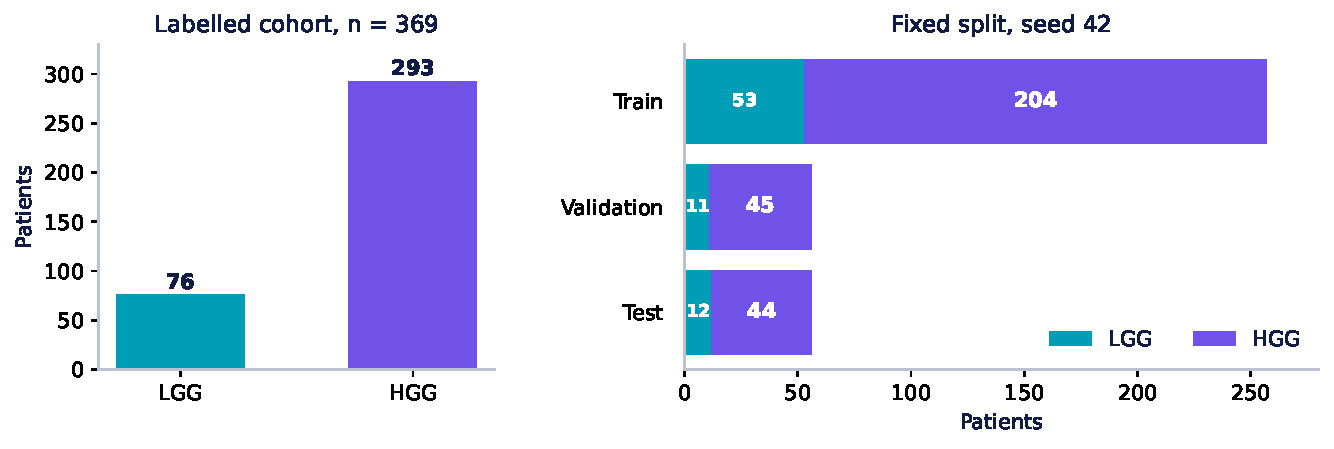
\includegraphics[width=\linewidth]{cohort.pdf}
\caption[Class distribution and fixed patient split]{Class distribution and fixed patient split derived from the saved manifest. Every count denotes a patient, not an image slice.}
\label{fig:cohort}
\end{figure}

\section{Patient partitions}
The fixed stratified split uses seed 42 and contains 257 training, 56 validation and 56 test patients. Table~\ref{tab:split} gives the class counts. The ROI and whole-brain experiments use the same assignments so that their fixed-test results refer to identical patients.
\begin{table}[htbp]
\centering
\caption{Fixed split used for both ROI and whole-brain experiments.}
\label{tab:split}
\begin{tabular}{lrrr}
\toprule
Partition & LGG & HGG & Total\\\midrule
Training & 53 & 204 & 257\\
Validation & 11 & 45 & 56\\
Test & 12 & 44 & 56\\\midrule
Total & 76 & 293 & 369\\\bottomrule
\end{tabular}
\end{table}

Five stratified patient folds are also recorded for rotating evaluation. Each rotation uses a separate test fold and validation fold, with the remaining three folds used for training. These assignments are described in Section~\ref{sec:cv}. Augmentation is applied only after partitioning and only to training samples.

\section{Visual inspection and cache traceability}
Preprocessing QA panels show the same anatomical location across the four channels and an overlay of the resized mask. Figure~\ref{fig:mri} is a real training-patient example from the recorded QA outputs. It documents the processed representation rather than serving as an independent diagnostic annotation.

\begin{figure}[htbp]
\centering
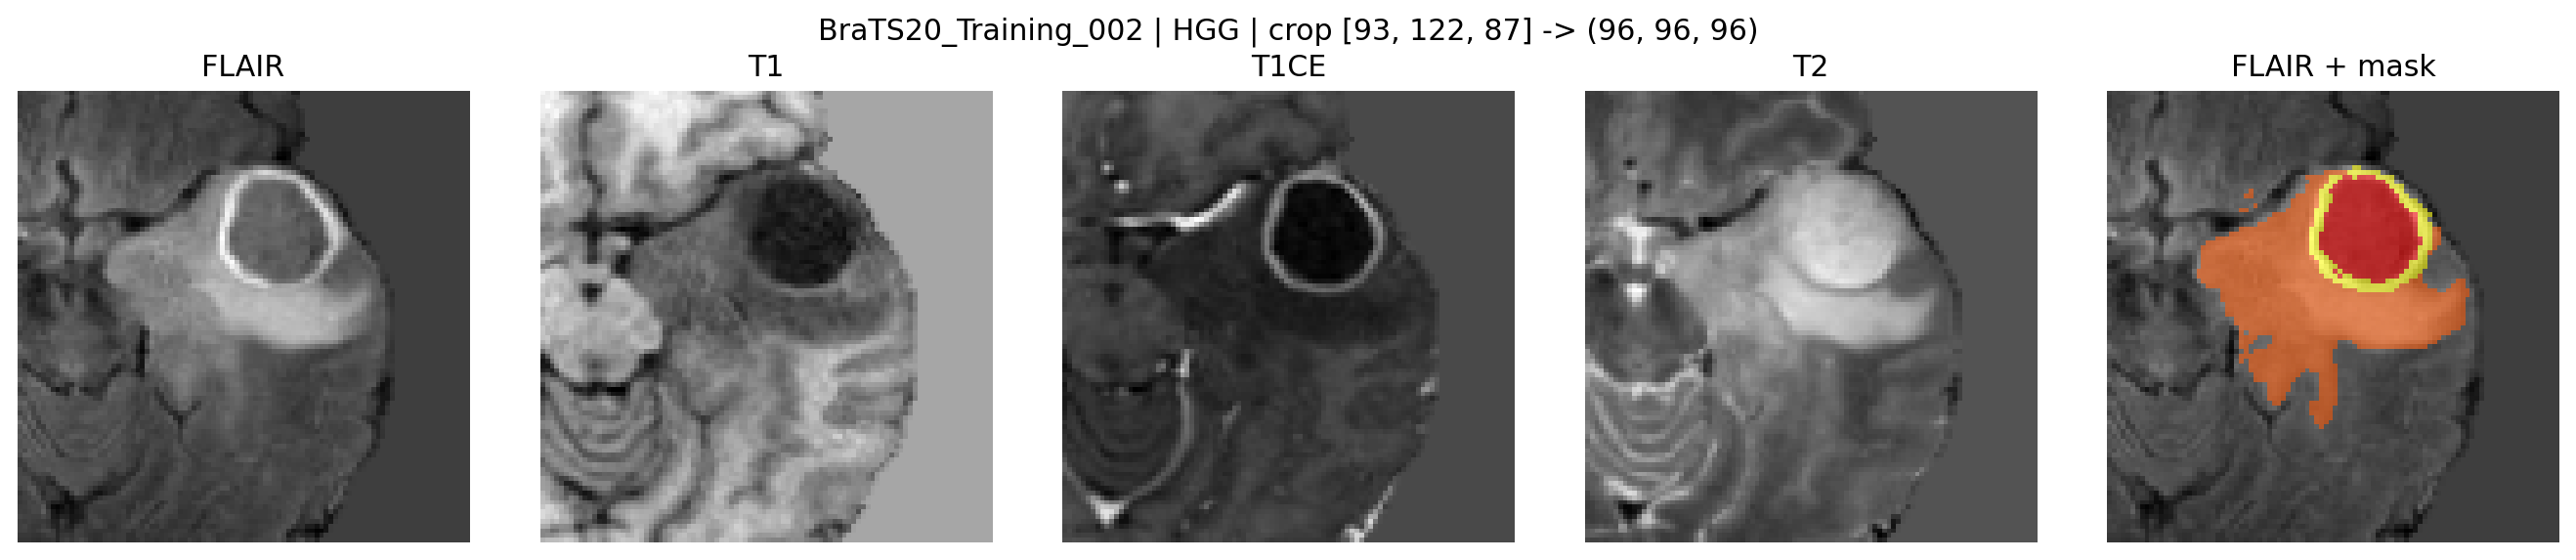
\includegraphics[width=\linewidth]{mri_example.png}
\caption[Real MRI preprocessing example]{Recorded preprocessing QA for training patient BraTS20\_Training\_002. The four MRI channels remain spatially aligned; the supplied mask is retained for inspection and ROI definition.}
\label{fig:mri}
\end{figure}

Each compressed cache stores the image tensor, target and preprocessing metadata. Metadata include source-file SHA-256 hashes, original geometry, orientation, crop bounds and normalization statistics. Cache images are stored in float16 and converted to float32 when loaded. The dataset loader verifies cached-label agreement and rejects missing cache files. These records support traceability from a processed sample back to its source volumes.

\FloatBarrier
\chapter[Methodology and Experimental Design]{Methodology and\\Experimental Design}
\label{ch:methods}
\section{Processing pipeline}
Figure~\ref{fig:pipeline} summarizes the implemented pipeline. The same preprocessing configuration saved in a checkpoint is applied during inference, so the predicted patient uses the modality order and crop specification used for training.

\begin{figure}[H]
\centering
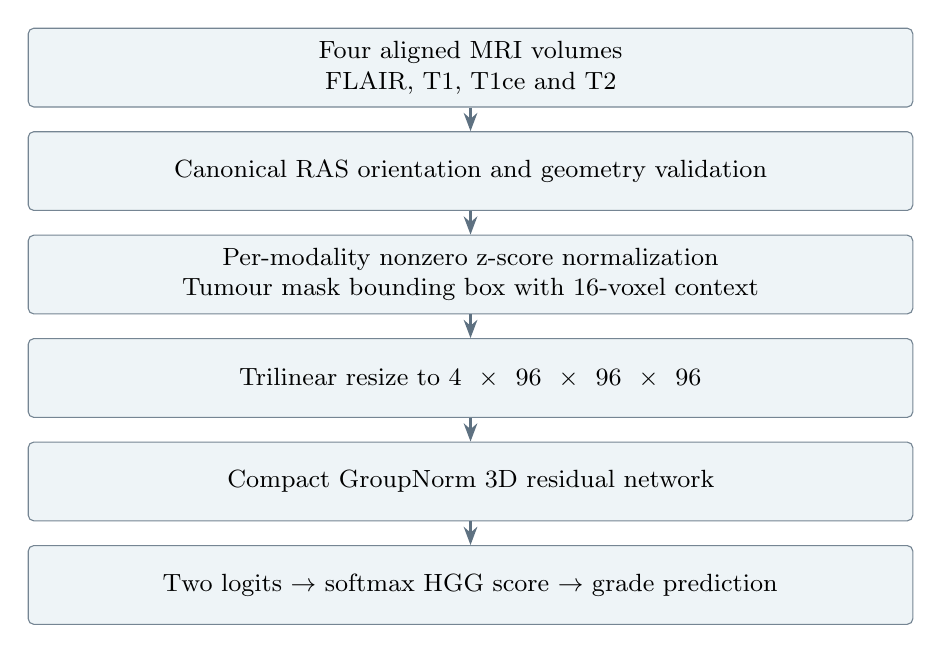
\begin{tikzpicture}[node distance=3mm,>=Stealth,
box/.style={draw=navy!60,fill=pale,rounded corners=2pt,text width=110mm,align=center,minimum height=10mm,font=\small}]
\node[box] (a) {Four aligned MRI volumes\\FLAIR, T1, T1ce and T2};
\node[box,below=of a] (b) {Canonical RAS orientation and geometry validation};
\node[box,below=of b] (c) {Per-modality nonzero z-score normalization\\Tumour mask bounding box with 16-voxel context};
\node[box,below=of c] (d) {Trilinear resize to $4\times96\times96\times96$};
\node[box,below=of d] (e) {Compact GroupNorm 3D residual network};
\node[box,below=of e] (f) {Two logits $\rightarrow$ softmax HGG score $\rightarrow$ grade prediction};
\foreach \s/\t in {a/b,b/c,c/d,d/e,e/f} \draw[->,thick,navy!70] (\s)--(\t);
\end{tikzpicture}
\caption[Patient-level ROI processing pipeline]{Implemented ROI pipeline. The mask supplies localization and is not an additional classifier input channel.}
\label{fig:pipeline}
\end{figure}

\subsection{Orientation and intensity normalization}
Volumes are loaded in canonical RAS orientation and checked for matching geometry. Each modality is standardized independently using its own nonzero foreground before cropping. For modality $m$ with nonzero voxel set $\Omega_m$,
\begin{equation}
\mu_m=\frac{1}{|\Omega_m|}\sum_{v\in\Omega_m}I_m(v),\qquad
\sigma_m=\sqrt{\frac{1}{|\Omega_m|}\sum_{v\in\Omega_m}(I_m(v)-\mu_m)^2},
\end{equation}
The standardized intensity is
\begin{equation}
\widetilde I_m(v)=\begin{cases}(I_m(v)-\mu_m)/\sigma_m,&v\in\Omega_m,\\0,&v\notin\Omega_m.\end{cases}
\end{equation}
Empty foregrounds and near-zero variance cause an error. Statistics are calculated within each patient rather than fitted jointly across the cohort, so no training-set intensity estimator is applied to held-out patients.

\subsection{Cropping and interpolation}
For the main experiment, the crop is the axis-aligned bounding box of $S_i>0$, expanded by 16 voxels in every direction and clipped to image bounds. The normalized crop is resized to \roi{} using trilinear interpolation. The mask is resized with nearest-neighbour interpolation for QA, preserving discrete labels.

The whole-brain experiment instead crops the union of the nonzero foregrounds of the four MRI volumes, with zero margin. It uses the same final tensor size. Because the two inputs represent different fields of view, a voxel in the resized tensor does not necessarily correspond to 1~mm of original anatomy. Resizing to a cube can also alter relative spatial proportions. These are properties of the selected baseline representation.

\section{Compact 3D residual architecture}
The network uses a $5\times5\times5$ convolutional stem, followed by GroupNorm, ReLU and max pooling. Four stages contain two residual blocks each. Every block uses two $3\times3\times3$ convolutions, with GroupNorm after each convolution. A projected shortcut is used when the stage changes shape. Table~\ref{tab:architecture} lists the tensor dimensions for a single patient; the batch dimension is omitted.

\begin{table}[H]
\centering
\caption{Architecture of the main width-16 model. GN uses eight groups.}
\label{tab:architecture}
\small
\begin{tabularx}{\linewidth}{lYr}
\toprule
Component & Operation & Output shape\\\midrule
Input & Four MRI modalities & $4\times96^3$\\
Stem & $5^3$ convolution, stride 2; GN; ReLU & $16\times48^3$\\
Pooling & $3^3$ max pool, stride 2 & $16\times24^3$\\
Stage 1 & Two residual blocks, width 16 & $16\times24^3$\\
Stage 2 & Two blocks, width 32; first stride 2 & $32\times12^3$\\
Stage 3 & Two blocks, width 64; first stride 2 & $64\times6^3$\\
Stage 4 & Two blocks, width 128; first stride 2 & $128\times3^3$\\
Head & Global average pool; dropout 0.30 & $128$\\
Classifier & Linear $128\rightarrow2$ & $2$ logits\\\bottomrule
\end{tabularx}
\end{table}

The model contains 2,081,186 trainable parameters. Global average pooling avoids a large spatial fully connected layer, while dropout regularizes the final representation. The channel widths are chosen to keep the baseline manageable on the recorded GPU. No pretrained weights are loaded.

\begin{figure}[H]
\centering
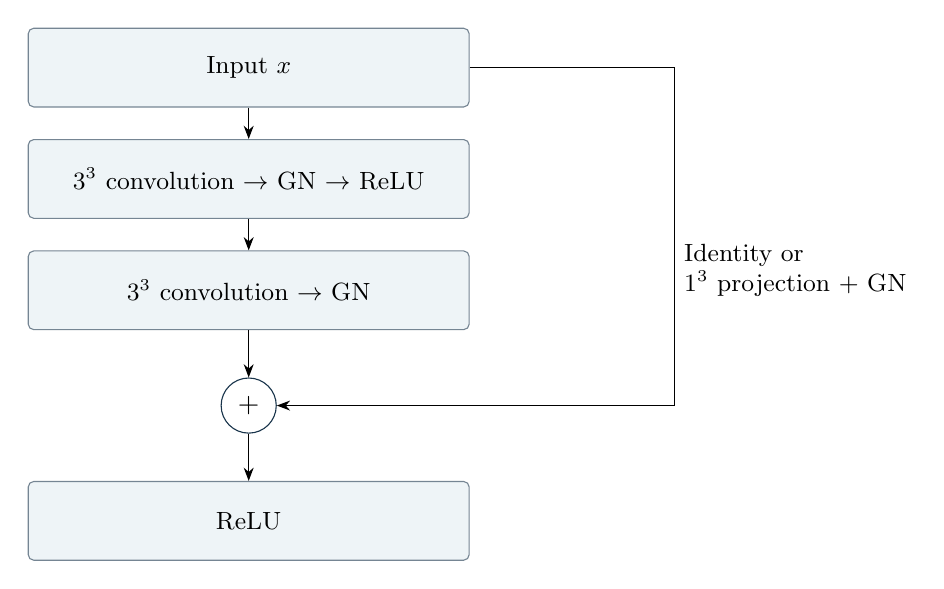
\begin{tikzpicture}[>=Stealth,node distance=4mm,
b/.style={draw=navy!60,fill=pale,rounded corners=2pt,minimum width=56mm,minimum height=10mm,align=center,font=\small}]
\node[b] (x) {Input $x$};
\node[b,below=of x] (c1) {$3^3$ convolution $\rightarrow$ GN $\rightarrow$ ReLU};
\node[b,below=of c1] (c2) {$3^3$ convolution $\rightarrow$ GN};
\node[draw=navy,circle,below=6mm of c2,minimum size=7mm] (sum) {$+$};
\node[b,below=6mm of sum] (out) {ReLU};
\draw[->] (x)--(c1);\draw[->] (c1)--(c2);\draw[->] (c2)--(sum);\draw[->] (sum)--(out);
\draw[->] (x.east)--++(26mm,0) |- node[pos=.3,right,font=\small,align=left] {Identity or\\$1^3$ projection + GN} (sum.east);
\end{tikzpicture}
\caption[Basic 3D residual block]{Basic 3D residual block. Stage transitions use a projected shortcut and spatial downsampling in the first convolution.}
\label{fig:block}
\end{figure}

\section{Training procedure}
Training-only augmentation includes a left--right flip with probability 0.5, per-channel intensity scaling in $[0.9,1.1]$, and foreground Gaussian noise with standard deviation 0.03 applied with probability 0.5. Validation and test inputs are not augmented. The loader shuffles training patients and keeps deterministic patient records for evaluation.

Table~\ref{tab:training} summarizes the shared settings. A physical batch contains one patient. Gradients are accumulated over four steps before an optimizer update, except for a possible shorter final window. CUDA automatic mixed precision reduces activation memory use.

\begin{table}[H]
\centering
\caption{Settings used by the recorded main GPU experiments.}
\label{tab:training}
\begin{tabularx}{\linewidth}{lY}
\toprule
Setting & Value\\\midrule
Random seed & 42\\
Optimizer & AdamW; learning rate $2\times10^{-4}$; weight decay $10^{-4}$\\
Schedule & Cosine annealing, configured over 60 epochs\\
Batching & Physical batch 1; accumulation factor 4\\
Precision and clipping & CUDA AMP; gradient norm clipped to 5\\
Training limit & 60 epochs; early stopping patience 12\\
Checkpoint criterion & Highest validation balanced accuracy\\
Effective objective & Unweighted cross-entropy (see Section~\ref{sec:loss})\\
Compute & Recorded CUDA execution on a Tesla T4\\\bottomrule
\end{tabularx}
\end{table}

\subsection{Effective loss in the completed runs}
\label{sec:loss}
The source computes inverse-frequency class weights from the training partition and passes them to \texttt{CrossEntropyLoss}. Under the default mean reduction, the weighted terms are divided by the sum of the target weights~\cite{pytorchce}. For a one-patient microbatch,
\begin{equation}
\mathcal{L}_{\mathrm{mean}}=\frac{w_y[-\log p_\theta(y\mid X)]}{w_y}
=-\log p_\theta(y\mid X).
\label{eq:cancellation}
\end{equation}
The weight cancels before gradient accumulation. Thus the recorded runs are effectively unweighted cross-entropy experiments. This implementation finding was identified after training; the report does not attribute the results to successful class weighting. Appendix~\ref{app:loss} gives the implications and a proposed correction for a future, separately evaluated run.

The final partial accumulation window is also divided by the configured factor of four rather than its actual number of microbatches. Its update can consequently be smaller. The archived code is retained as the source of the reported results.

\subsection{Model selection and checkpoint contents}
After each epoch, validation balanced accuracy is compared with the best previous value. An improvement greater than $10^{-6}$ saves a checkpoint and resets the patience counter. Training stops after 12 epochs without improvement, or at the configured maximum. The selected checkpoint is reloaded before test prediction.

Checkpoints contain model state, model configuration, preprocessing configuration, class mapping and the selected epoch. They do not contain a complete optimizer, scheduler and scaler state for automatic training resumption. A saved best model can be used for inference; it is not a full recovery point for an interrupted training trajectory.

\section{Patient-level evaluation}
\label{sec:cv}
The fixed split supports development and the matched ROI/whole-brain comparison. The additional five-fold procedure fits a new model for each rotation. If $k$ is the test fold, validation uses $(k+1)\bmod5$ and training uses the other three folds. Within each rotation, the training, validation and test patients are disjoint.

\begin{figure}[htbp]
\centering
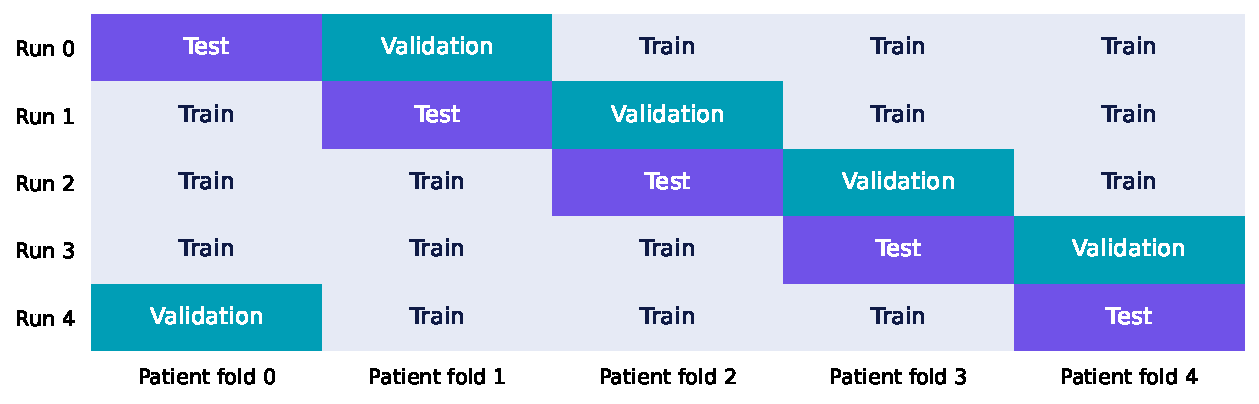
\includegraphics[width=\linewidth]{protocol.pdf}
\caption[Rotating train--validation--test protocol]{Rotating train--validation--test protocol. Each row is a separate model fit; each patient belongs to exactly one outer test fold.}
\label{fig:protocol}
\end{figure}

\begin{table}[htbp]
\centering
\caption{Class counts in the five rotations, shown as LGG/HGG.}
\label{tab:foldcounts}
\begin{tabular}{crrr}
\toprule
Test fold & Training & Validation & Test\\\midrule
\tableinput fold_counts.tex
\bottomrule
\end{tabular}
\end{table}

The resulting test predictions cover all 369 patients exactly once. The protocol is a rotating three-role evaluation with roughly 60\% training, 20\% validation and 20\% test data per run. It is not a conventional fit on four full folds with no separate validation partition, and no nested hyperparameter search was conducted.

\section{Metrics and aggregation}
With HGG as the positive class, TP and FN refer to HGG and TN and FP to LGG. The reported measures are
\begin{align}
\mathrm{Accuracy}&=\frac{\mathrm{TP}+\mathrm{TN}}{N},\\
\mathrm{Sensitivity}_{\mathrm{HGG}}&=\frac{\mathrm{TP}}{\mathrm{TP}+\mathrm{FN}},\qquad
\mathrm{Specificity}_{\mathrm{LGG}}=\frac{\mathrm{TN}}{\mathrm{TN}+\mathrm{FP}},\\
\mathrm{Balanced\ accuracy}&=\tfrac12\left(\mathrm{Sensitivity}_{\mathrm{HGG}}+\mathrm{Specificity}_{\mathrm{LGG}}\right),\\
\mathrm{Macro\mbox{-}F1}&=\tfrac12\left(F1_{\mathrm{LGG}}+F1_{\mathrm{HGG}}\right).
\end{align}
ROC-AUC evaluates the ranking of HGG scores across thresholds. It does not measure calibration. Classification metrics use the fixed 0.5 decision rule; no validation-based threshold tuning or calibration study was performed.

Pooled OOF metrics are calculated once from all 369 held-out predictions. Mean fold metrics are the unweighted average of the five test-fold scores. Their sample SD uses denominator $5-1$. Pooled and mean fold metrics need not agree, especially for AUC, because pooled ranking compares scores from separately fitted models. Fold SD describes variation across the recorded partitions; it is not a confidence interval.

\section{Implementation checks}
An eight-patient memorization check uses only the fixed training partition, with four examples per class. A smaller width-four model and zero dropout reach 100\% training accuracy and loss 0.01994 after 47 epochs. Reloaded checkpoint predictions match. This is a debugging check of learning and serialization, not a held-out performance result for the main width-16 model.

Post-run verification recomputes metrics from saved patient predictions, checks partition disjointness and OOF coverage, verifies label agreement, loads the seven main checkpoints and checks finite parameters. Histories are checked against the recorded checkpoint-selection criterion. These checks establish consistency of the delivered artifacts; they do not constitute an independent repeat of the full GPU training process.

\FloatBarrier
\chapter{Results}
\label{ch:results}
\section{Overview of completed experiments}
The frozen GPU export contains seven main model fits: one fixed-split ROI model, five ROI cross-validation models, and one fixed-split whole-brain model. All use four MRI channels, \roi{} inputs and base width 16. Table~\ref{tab:mainresults} reports their recorded test metrics.

\begin{table}[htbp]
\centering
\caption{Completed GPU experiments. Percentages are used except for AUC. The pooled OOF row uses a different evaluation scheme from the fixed-split rows.}
\label{tab:mainresults}
\small
\begin{tabularx}{\linewidth}{Yrrrrr}
\toprule
Experiment & $n$ & Acc. & Bal. acc. & Macro-F1 & AUC\\\midrule
ROI fixed split & 56 & 83.93 & 71.59 & 73.63 & 0.8097\\
ROI pooled OOF & 369 & 87.26 & 84.67 & 81.96 & 0.8815\\
Whole-brain fixed & 56 & 75.00 & 65.91 & 64.94 & 0.7936\\\bottomrule
\end{tabularx}
\end{table}

The primary internal estimate is the pooled ROI OOF result because every cohort patient contributes one held-out prediction. It is interpreted together with fold variation and class-specific performance, rather than as a replacement for the fixed-split result.

\section{Fixed-split performance}
The ROI model selects epoch 10 using validation balanced accuracy of 87.58\% and stops after epoch 22. On the 56-patient test set it correctly classifies 47 patients, giving 83.93\% accuracy. Its confusion matrix is
\begin{equation}
C_{\mathrm{ROI,fixed}}=\begin{pmatrix}6&6\\3&41\end{pmatrix},
\end{equation}
where rows and columns are ordered LGG, HGG. HGG recall is $41/44=93.18\%$, whereas LGG recall is $6/12=50.00\%$. Balanced accuracy of 71.59\% therefore gives a more cautious account than overall accuracy alone. A single additional correct LGG prediction would change fixed-test LGG recall by 8.33 percentage points.

The saved checkpoint was reloaded for a held-out-patient inference demonstration and returned HGG with score 0.98386. This verifies checkpoint-to-prediction execution on a cohort test patient. It is not an independent external sample, and the softmax score is not a calibrated probability of diagnostic correctness.

\section{Five-fold ROI evaluation}
\subsection{Pooled predictions}
Across the 369 OOF predictions, 322 patients are correctly classified. The pooled confusion matrix is
\begin{equation}
C_{\mathrm{OOF}}=\begin{pmatrix}61&15\\32&261\end{pmatrix}.
\label{eq:pooledcm}
\end{equation}
Thus 61 of 76 LGG patients and 261 of 293 HGG patients are recognized. Table~\ref{tab:classresults} gives the class-specific measures.

\begin{table}[htbp]
\centering
\caption{Class-specific performance from pooled ROI OOF predictions.}
\label{tab:classresults}
\begin{tabular}{lrrrr}
\toprule
Class & Support & Precision (\%) & Recall (\%) & F1 (\%)\\\midrule
LGG & 76 & 65.59 & 80.26 & 72.19\\
HGG & 293 & 94.57 & 89.08 & 91.74\\\bottomrule
\end{tabular}
\end{table}

The model makes 15 LGG-to-HGG errors and 32 HGG-to-LGG errors. LGG precision remains lower because 32 HGG cases enter the predicted-LGG group. Reporting both recalls and macro-F1 therefore exposes differences that overall accuracy can conceal.

\begin{figure}[htbp]
\centering
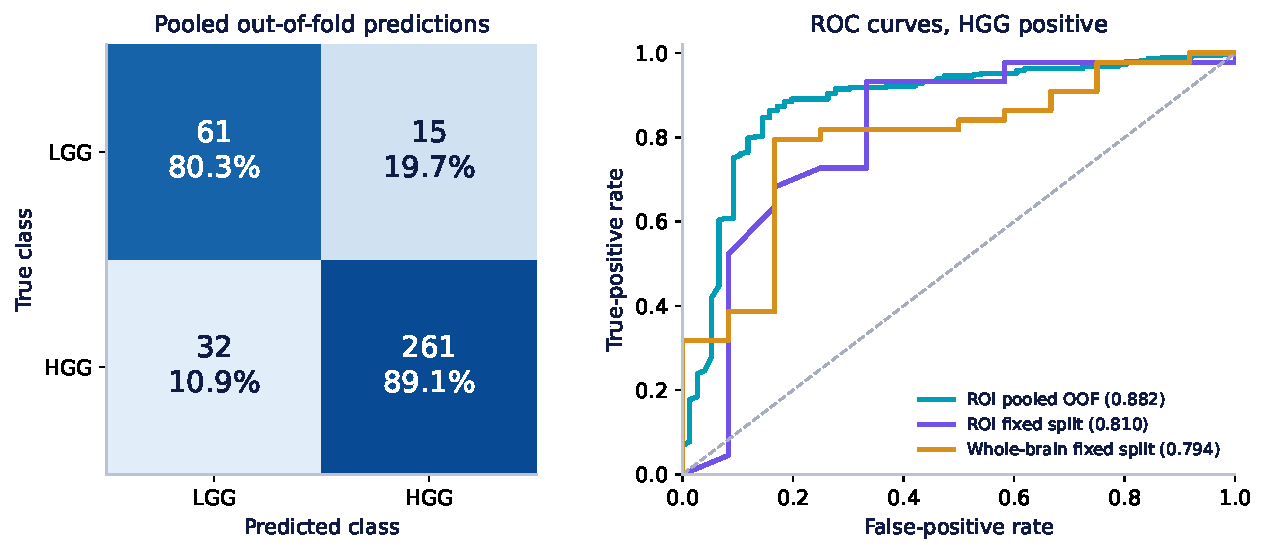
\includegraphics[width=\linewidth]{pooled_results.pdf}
\caption[Pooled ROI confusion matrix and ROC curves]{Pooled ROI confusion matrix and empirical ROC curves. The confusion matrix shows counts and percentages within each true class. Fixed-split and pooled curves refer to different evaluation populations and model fits.}
\label{fig:pooled}
\end{figure}

An always-HGG classifier would achieve 79.40\% accuracy and 50.00\% balanced accuracy on this full cohort. The pooled ROI predictions improve accuracy by 7.86 percentage points and recover 80.26\% of LGG cases. The results therefore demonstrate learning beyond the majority-class decision, while remaining an internal estimate on this selected cohort.

\subsection{Performance across folds}
Table~\ref{tab:foldresults} reports every test fold rather than selecting the most favourable run. Mean fold balanced accuracy is 84.57\% with SD 5.65 percentage points. Mean macro-F1 is 81.87\% with SD 4.40 percentage points.

\begin{table}[htbp]
\centering
\caption{Held-out ROI fold results. Metric columns other than AUC are percentages.}
\label{tab:foldresults}
\small
\begin{tabular}{crrrrrr}
\toprule
Fold & $n$ & Bal. acc. & Macro-F1 & HGG recall & LGG recall & AUC\\\midrule
\tableinput fold_metrics.tex
\bottomrule
\end{tabular}
\end{table}

\begin{figure}[htbp]
\centering
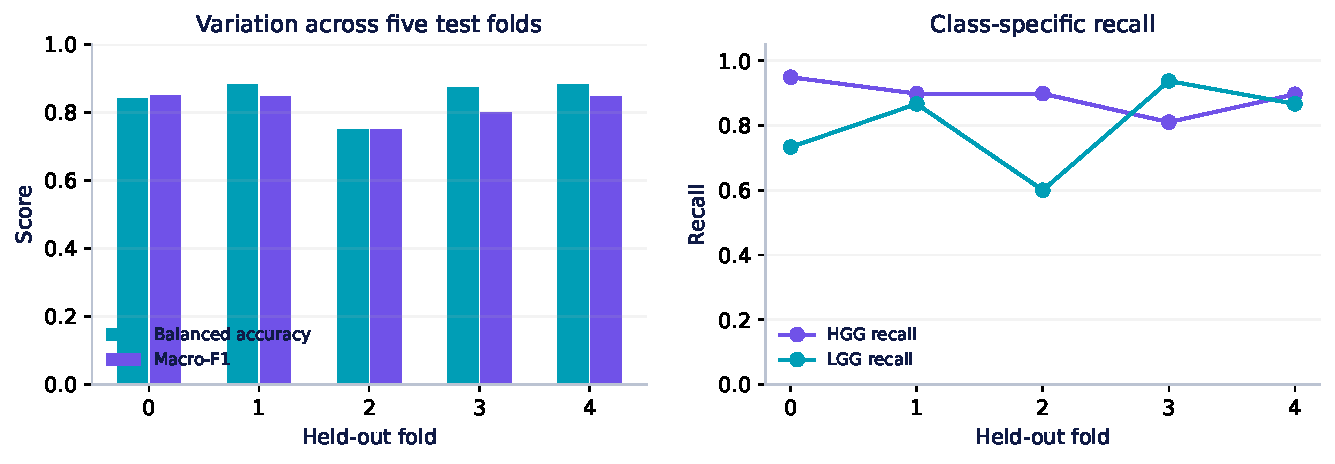
\includegraphics[width=\linewidth]{fold_results.pdf}
\caption[Performance variation across the five test folds]{Variation across the five held-out ROI folds. LGG recall ranges from 60.00\% to 93.75\%, showing sensitivity to the patient partition.}
\label{fig:foldresults}
\end{figure}

Fold 2 has the lowest balanced accuracy, 74.92\%, with LGG recall of 60.00\%. Fold 3 reaches 93.75\% LGG recall but 81.03\% HGG recall. This trade-off would be obscured by reporting a single best-fold score. The models share many training patients, and only seed 42 was used; the five scores are not independent repetitions of the entire study.

\subsection{Pooled versus mean fold AUC}
The pooled OOF AUC is 0.8815. The mean fold AUC is 0.9008 with sample SD 0.0261. Within-fold AUC compares scores produced by one fitted model. Pooled AUC additionally compares scores across models, whose output scales may differ. Both quantities are valid descriptions of the saved predictions, but they answer different ranking questions and must retain their aggregation labels.

\section{Training dynamics and compute}
Figure~\ref{fig:training} shows fixed-split training and validation losses. For the ROI model, training loss falls while validation loss fluctuates after the selected epoch. The later reduction in training loss does not reliably improve validation balanced accuracy. The whole-brain run selects epoch 6 and stops at epoch 18.

\begin{figure}[htbp]
\centering
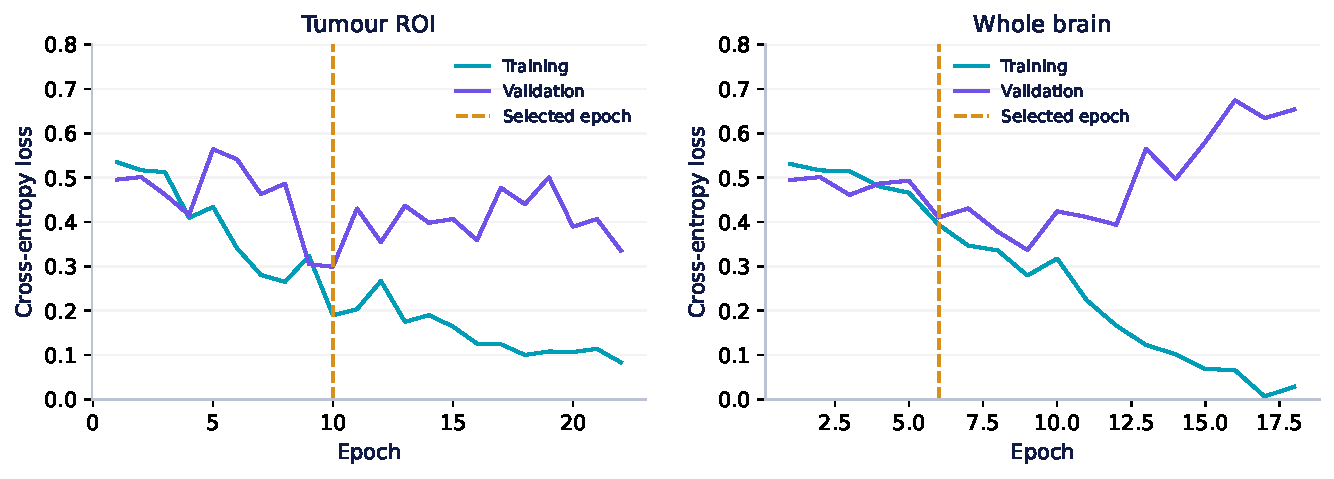
\includegraphics[width=\linewidth]{training.pdf}
\caption[Fixed-split training and validation loss histories]{Recorded fixed-split loss histories. Dashed lines identify the validation-balanced-accuracy checkpoint, which need not be the minimum-validation-loss epoch.}
\label{fig:training}
\end{figure}

\begin{table}[htbp]
\centering
\caption{Selected checkpoints and recorded training durations. Download and preprocessing are excluded from these timers.}
\label{tab:runtime}
\begin{tabular}{lrrr}
\toprule
Run & Selected epoch & Stop epoch & Minutes\\\midrule
ROI fixed & 10 & 22 & 9.69\\
CV fold 0 & 22 & 34 & 13.18\\
CV fold 1 & 11 & 23 & 9.17\\
CV fold 2 & 29 & 41 & 15.98\\
CV fold 3 & 9 & 21 & 8.15\\
CV fold 4 & 19 & 31 & 12.50\\
Whole-brain fixed & 6 & 18 & 7.73\\\bottomrule
\end{tabular}
\end{table}

The fixed ROI model takes 581.64 seconds, the five ROI fits together take 3,539.85 seconds (approximately 59.00 minutes), and the whole-brain model takes 464.09 seconds. These durations describe the recorded Tesla T4 session and should not be treated as guarantees for another runtime.

\section{Matched ROI and whole-brain comparison}
On the same fixed test patients, the whole-brain confusion matrix is
\begin{equation}
C_{\mathrm{brain,fixed}}=\begin{pmatrix}6&6\\8&36\end{pmatrix}.
\end{equation}
Compared with the ROI model, five additional HGG patients are misclassified and the LGG counts are unchanged. ROI therefore improves HGG recall from 81.82\% to 93.18\%, while LGG recall remains 50.00\%. Balanced accuracy rises from 65.91\% to 71.59\%, and AUC from 0.7936 to 0.8097.

\begin{figure}[htbp]
\centering
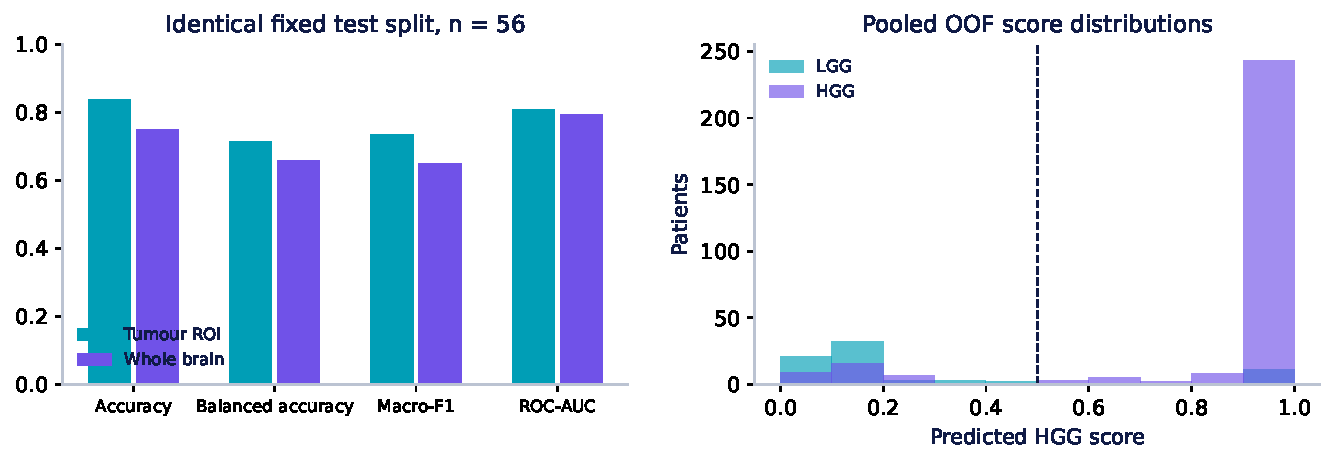
\includegraphics[width=\linewidth]{cropping_scores.pdf}
\caption[Matched crop comparison and OOF score distributions]{Left: matched fixed-split crop comparison. Right: HGG score distributions for pooled ROI OOF predictions. Score distributions are descriptive and do not establish probability calibration.}
\label{fig:cropping}
\end{figure}

The matched result favours ROI under the executed settings. Localization may emphasize tumour tissue and preserve its relative scale after resizing, but these mechanisms are hypotheses. Crop definition and margin change together, only one split is tested, and ROI has access to a supplied expert mask. The pooled ROI row in Table~\ref{tab:mainresults} is not used as a controlled comparator for the fixed whole-brain row.

\FloatBarrier
\chapter{Discussion and Limitations}
\label{ch:discussion}
\section{What the experiments establish}
The project demonstrates a working path from genuine multimodal volumes to patient-level held-out predictions. Cohort validation, preprocessing, cached tensors, supervised learning, checkpoint selection and inference are connected in one implementation. The saved predictions support useful internal discrimination: pooled balanced accuracy is 84.67\%, and both classes are recognized beyond a majority-class rule.

The primary result nevertheless needs its full context. The fixed ROI model recognizes only half of its LGG test patients. Fold-wise LGG recall ranges from 60.00\% to 93.75\%. The pooled value summarizes several fitted models and patient assignments; it is not evidence that a single deployed model improved from the fixed-split result to the pooled result.

\section{Class imbalance and implementation findings}
The cohort contains approximately 3.86 HGG patients for each LGG patient. Balanced accuracy and macro-F1 are consequently central to evaluation. The post-run loss audit shows that the intended inverse-frequency weighting did not affect singleton mean-reduced losses. The observed performance is therefore evidence for the effective unweighted procedure, not for a successful weighting strategy.

Correcting the loss is a priority for continuation, but such a correction creates a new experiment. It should use an explicit development protocol and preserve the original artifacts for comparison. The same applies to correcting partial-window gradient scaling. Neither code change can be retroactively associated with the existing checkpoints.

\section{Segmentation dependence and spatial representation}
ROI preprocessing uses a supplied segmentation to identify the tumour region. This is useful annotation-derived localization, even though the mask is not a model channel. Applying the ROI classifier to a new examination would require a suitable manual mask or a separately evaluated segmentation system. The current pipeline does not provide an automated segmentation model.

Resizing both localized and whole-brain crops to the same cube also changes their spatial scale. The experiment does not isolate localization, background reduction, tumour size or interpolation distortion. A matched multi-fold comparison and alternative spatial representations would be needed to investigate these factors systematically.

\section{Generalization and statistical scope}
The evaluation is internal to one selected public cohort. No external hospital data, held-out-site experiment or prospective study is available. Patient-ID disjointness prevents a specific form of overlap within each fit, but does not establish scanner or institution independence.

Only one seed was evaluated. Fold SD describes the recorded patient partitions and is not a confidence interval. No repeated-seed analysis, calibration study, significance test or uncertainty model was conducted. The small LGG test counts make class recall particularly sensitive to individual patients.

The target labels are the dataset's legacy HGG/LGG categories. The results should not be extended to contemporary molecular classification or unrelated tumour types. Softmax scores are uncalibrated research outputs, and the study does not establish clinical utility or safety.

\section{Relationship to the earlier 2D work}
The earlier project uses image folders and a different four-class task. The present work uses four aligned volumes for a binary grade label at patient level. Differences in data, target definition and evaluation rules prevent a direct ranking of the two approaches by accuracy. The completed contribution is a volumetric experimental foundation rather than a demonstrated improvement on an identical benchmark.

\chapter{Conclusion and Future Work}
\label{ch:conclusion}
This B.Tech Project I implements and evaluates a compact 3D MRI classifier on all 369 labelled patients in the selected BraTS 2020 cohort. The pipeline preserves patient identity, validates image geometry, processes four modalities and selects models using a separate validation partition.

The main ROI experiment achieves 87.26\% pooled OOF accuracy, 84.67\% balanced accuracy, 81.96\% macro-F1 and 0.8815 AUC. Mean fold balanced accuracy is 84.57\% with SD 5.65 percentage points. A matched fixed-split comparison favours ROI over whole-brain input in the recorded setting. The results establish a functioning internal baseline, while minority-class variation and mask dependence limit broader interpretation.

The implementation audit identifies class-weight cancellation at physical batch size one. Reporting this effective objective is necessary to describe what was actually trained. The measured predictions remain unchanged, and a corrected objective remains a new experimental step.

\section{Priorities for continuation}
\begin{enumerate}
\item Correct the weighted-loss reduction and final accumulation-window scaling, then assess them under a declared development procedure.
\item Repeat ROI and whole-brain evaluation using matched folds and additional seeds.
\item Study validation-based calibration and threshold selection if a downstream research objective requires them.
\item Evaluate volumetric transfer learning or self-supervised pretraining against the corrected supervised baseline.
\item Add site-aware or external evaluation when a suitable independent cohort is available, and evaluate automatic segmentation before using it for ROI inference.
\end{enumerate}
The present deliverables provide the source code, executed evidence, checkpoints, patient predictions and documented limitations required to review the completed baseline and plan the next stage.

\appendix
\chapter{Reproducibility and Artifact Record}
\label{app:repro}
\section{Evidence underlying this report}
The numerical results come from the supplied executed Colab notebook and frozen GPU export. Table~\ref{tab:artifacts} identifies the principal evidence files relative to the extracted results directory. The report's scientific figures are derived from these saved metrics and predictions. No new GPU training was performed while preparing this review draft.

\begin{table}[htbp]
\centering
\caption{Principal files in the frozen GPU results export.}
\label{tab:artifacts}
\small
\begin{tabularx}{\linewidth}{>{\raggedright\arraybackslash}p{64mm}Y}
\toprule
Artifact & Purpose\\\midrule
\nolinkurl{manifest.csv}, \nolinkurl{data_audit.csv} & Cohort, labels, partitions and geometry checks\\
\nolinkurl{fixed_split/} & ROI checkpoint, history, predictions and test metrics\\
\nolinkurl{cv5/fold_0/} through \nolinkurl{cv5/fold_4/} & Per-fold checkpoints, histories and evaluations\\
\nolinkurl{cv5/out_of_fold_predictions.csv} & One held-out prediction for each patient\\
\nolinkurl{cv5/cross_validation_metrics.json} & Pooled metrics and fold summaries\\
\nolinkurl{whole_brain_fixed/} & Matched whole-brain experiment\\
\nolinkurl{source_code.zip} & Executed implementation snapshot\\
\nolinkurl{environment.txt}, \nolinkurl{gpu.txt} & Recorded packages and GPU information\\\bottomrule
\end{tabularx}
\end{table}

\section{Environment and reconstruction}
The saved environment records Python 3.13 in Colab, PyTorch 2.11.0+cu130, NumPy 2.1.3, pandas 2.2.3, nibabel 5.4.2 and scikit-learn 1.6.1, with a Tesla T4 device. Exact numerical reproduction can depend on software versions and GPU kernels.

To reconstruct the pipeline, restore the source and grade mapping, obtain the original MRI cohort, build and audit the manifest, generate ROI96 caches, inspect QA and run the training-only debugging check. The main experiments then run in the order fixed ROI, five-fold ROI and fixed whole-brain. Saved prediction CSVs allow metric recalculation without rerunning training.

Raw MRI and processed cache tensors are excluded from the results ZIP. Absolute \nolinkurl{/content/} paths in manifests need rebuilding or remapping on another machine. A CSV manifest alone does not restore its referenced volumes. The original dataset is retained separately in the local BTP workspace.

\section{Notebook presentation and research record}
The unmodified executed notebook preserves the original setup history, including failed download attempts followed by the successful cache-bypass download. A cleaned review copy removes duplicate failed cells, consolidates setup code and corrects stale explanatory comments. Its retained training, evaluation, inference and QA outputs are preserved from the original record; it is explicitly labelled as an edited record rather than a new execution.

A separate fresh-run notebook has cleared outputs and writes to a timestamped directory to protect archived results. It retains the archived training objective for reproduction and discloses the loss issue. A future corrected-loss study must use a separately identified implementation and results directory.

\section{Assistance and review status}
AI assistance supported code development, debugging, artifact checks and preparation of the report and presentation. The student is responsible for reviewing the content, understanding the method and results, and meeting the Institute's attribution and disclosure requirements. This document is a review draft. Student and supervisor signature fields remain blank.

\chapter{Loss Reduction and Accumulation Audit}
\label{app:loss}
For a batch $\mathcal B$ of class-index targets, the implemented weighted mean cross-entropy has the form~\cite{pytorchce}
\begin{equation}
\mathcal L(\mathcal B)=
\frac{\sum_{i\in\mathcal B}w_{y_i}\ell_i}{\sum_{i\in\mathcal B}w_{y_i}},
\qquad \ell_i=-\log p_\theta(y_i\mid X_i).
\end{equation}
With $|\mathcal B|=1$, this simplifies to $\ell_i$ for any positive class weight. Accumulating four such singleton gradients yields a scaled sum of unweighted gradients; it cannot recover weights removed inside each criterion call. On the fixed training split, the configured LGG/HGG weights are approximately 2.4245 and 0.6299, but their presence in a configuration file does not imply that they affected the effective objective.

A future implementation could explicitly define a per-patient weighted objective,
\begin{equation}
\mathcal L_{\mathrm{new}}=\frac{1}{M}\sum_{i=1}^{M}w_{y_i}\ell_i,
\end{equation}
using unreduced losses and a declared normalization convention. That convention differs from normalizing by the sum of class weights; either choice must be deliberate and checked against the intended objective. The correction should be verified with unequal weights and compared gradients before retraining.

The accumulated update also needs to account for the actual size of the final window. If a window contains $M<4$ patients, dividing every loss by four scales its average gradient by $M/4$. For the 257-patient fixed training set, the final window contains one patient. The archived implementation performs this smaller update. The report preserves that fact; it does not claim that a corrected run has been completed.

\clearpage
\renewcommand{\bibname}{References}
\addcontentsline{toc}{chapter}{References}
\begin{thebibliography}{9}
\small
\bibitem{brats2020} CBICA, University of Pennsylvania. \emph{Multimodal Brain Tumor Segmentation Challenge 2020: Data}. \url{https://www.med.upenn.edu/cbica/brats2020/data.html}.
\bibitem{menze} B. H. Menze et al. ``The Multimodal Brain Tumor Image Segmentation Benchmark (BRATS).'' \emph{IEEE Transactions on Medical Imaging}, vol. 34, no. 10, pp. 1993--2024, 2015. \href{https://doi.org/10.1109/TMI.2014.2377694}{doi:10.1109/TMI.2014.2377694}.
\bibitem{bakas} S. Bakas et al. ``Advancing The Cancer Genome Atlas glioma MRI collections with expert segmentation labels and radiomic features.'' \emph{Scientific Data}, vol. 4, article 170117, 2017. \href{https://doi.org/10.1038/sdata.2017.117}{doi:10.1038/sdata.2017.117}.
\bibitem{resnet} K. He, X. Zhang, S. Ren and J. Sun. ``Deep Residual Learning for Image Recognition.'' \emph{Proceedings of CVPR}, 2016. \url{https://arxiv.org/abs/1512.03385}.
\bibitem{groupnorm} Y. Wu and K. He. ``Group Normalization.'' \emph{Proceedings of ECCV}, 2018. \url{https://arxiv.org/abs/1803.08494}.
\bibitem{adamw} I. Loshchilov and F. Hutter. ``Decoupled Weight Decay Regularization.'' \emph{International Conference on Learning Representations}, 2019. \url{https://arxiv.org/abs/1711.05101}.
\bibitem{pytorchce} PyTorch Contributors. \emph{CrossEntropyLoss}, PyTorch 2.11 documentation. \url{https://docs.pytorch.org/docs/2.11/generated/torch.nn.CrossEntropyLoss.html}.
\end{thebibliography}
\end{document}
